
\subsection{Ballmaschine (Eruieren der Nenndrehzahl)}
\begin{figure}[h!]
	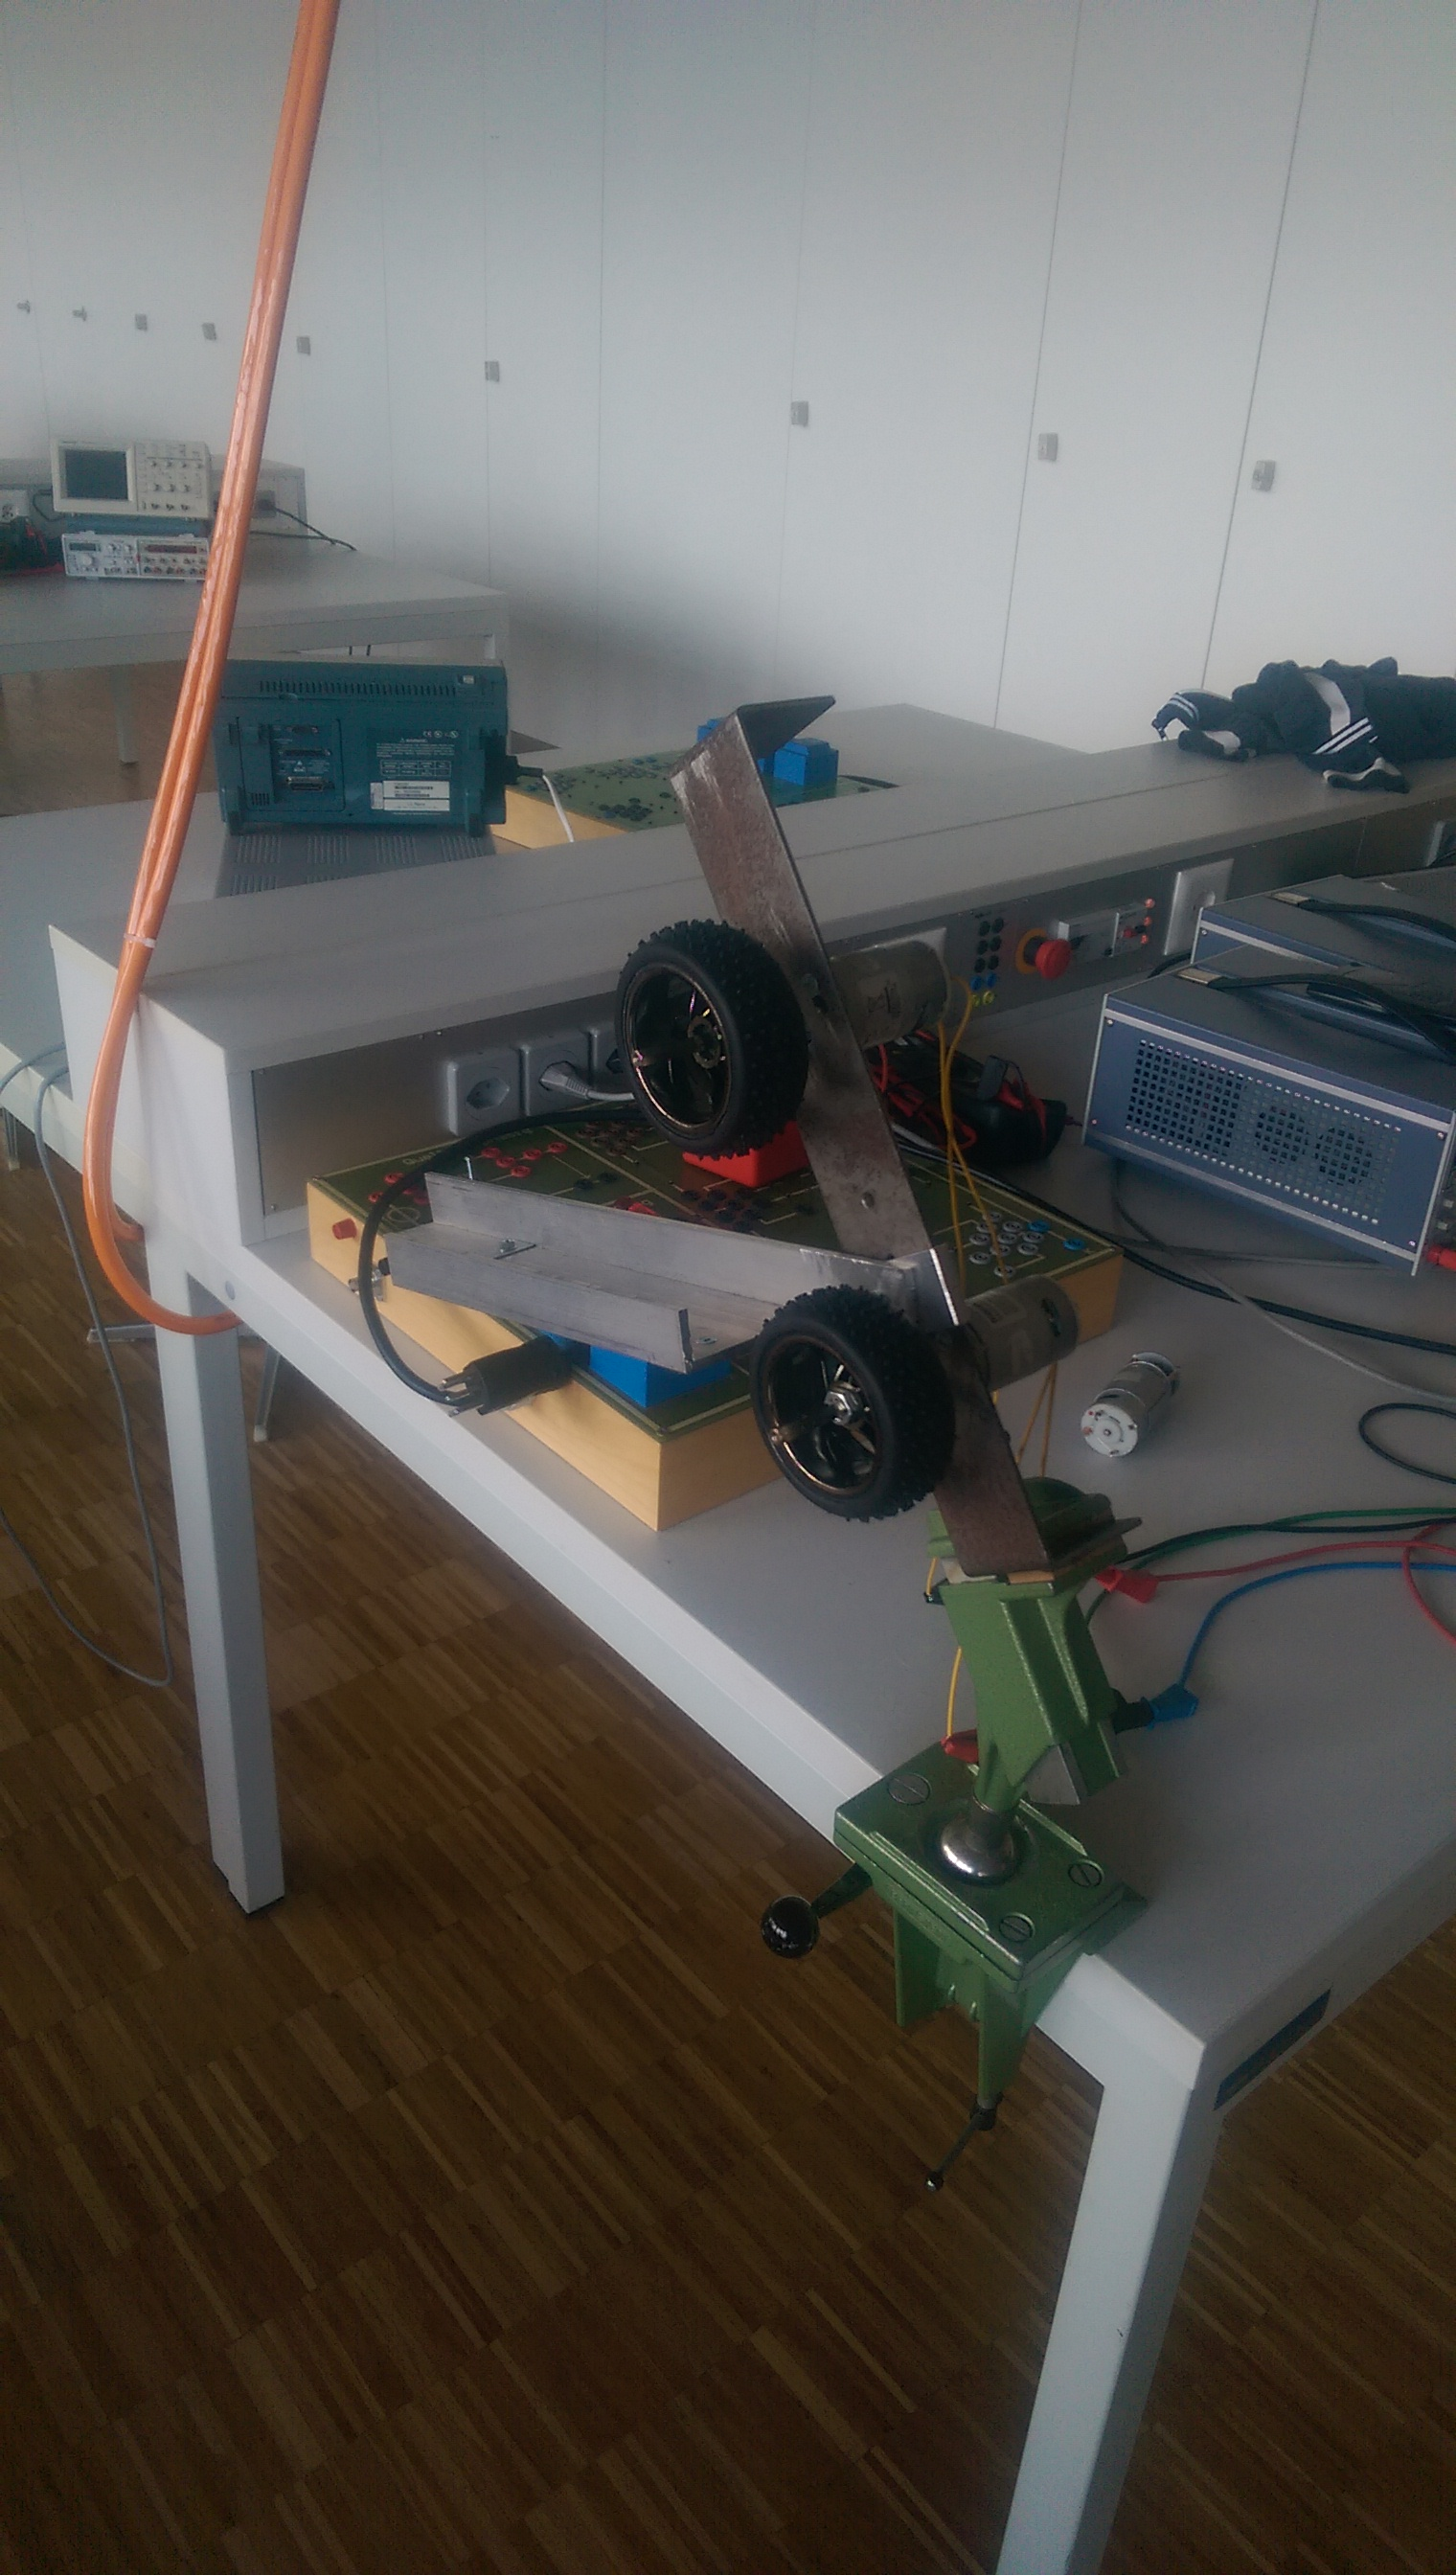
\includegraphics[width=5cm]{Funktionstests/Bilder/Ballmaschine_Drehzahl1.jpg}
	\centering
	\caption{Funktionsmuster Ballmaschine} 
\label{abb:Ballmaschine_Drehzahl}
\end{figure}	
\textit{Typ}: Ballmaschine \\ 
\textit{Datum}: 06.11.2014   \\
\textit{Ort}: Labor HSLU \\
\textit{Tester}: Matteo, Yves, Pascal \\
\textit{Ziel des Testes}:  Eruieren der Nenndrehzahl der DC-Motoren, Optimaler Wurfwinkel, Drehzahl der Schwungräder.  \\
\textit{Fazit / Verbesserungsvorschlag}: \\
Ballzuführung muss automatisiert gleichbleibend sein damit genaue Aussage über Wurfweite gemacht werden können. 
Unterschiedliche Tennisballmarken haben unterschiedliche Eigenschaften betreffend Wurfweite -> Fünf Bälle der „richtigen“ Marke kaufen. \\
\textit{Ziel erreicht}: Ja
